 \section{Hardware}
%metatekst til hardware
Dette afsnit skal være med til at dokumentere hardwaren i systemet \textit{the cell collector}, derfor indeholder afsnittet beskrivelser af systemets fysiske dele og deres funktionalitet. De fysiske deles specifikationer er uddybet og beskrevet i dette dokument. Der er begrundelser og argumenter for hvorfor de brugte komponenter er valgt.

\subsection{Læsevejledning til hardware}
%læsevejledning
Da dette afsnit er en udspecificering af hvilke specifikationer hardware komponenterne består af, ligger det sig tæt op af kravspecifikationen. Da det er kravene i kravspecifikationen, der ligger til grunde for de valgte hardware dele. I afsnittet findes der forskellige diagrammer der er med til at beskrive opbygningen, og kommunikationen af delene. Til hvert diagram vil der være en kort beskrivelse af hvad det beskriver. Hvert afsnit indeholder funktionalitet, specifikationer omkring det enkle komponent og begrundelser og argumentationer hvorfor det er valgt, i den skrevne rækkefølge. Afsnittene kan godt læses i dele, men for en komplet forståelse bør afsnittene læses i rækkefølge. 

%Det gamle afsnit, måske skal det være i et leverandør afsnit 
% Dette afsnit indeholder den nødvendige viden hardware delene i systemet Denne blok beskriver forbindelserne mellem diverse hardware med et internal block definition diagram. Dette diagram er med til at sikre at delene kan kommunikere sammen, uden unødvendige adaptere og omformere. Yderligere er der beskrevet hvordan information søgning, og viden er fundet omkring komponenterne. Primær kan det siges at hardware delene er fundet på Ebay.com(kilder til de konkrete sider?(måske under hvert produkt?)), for at hold budgettet i bund. Den manglende datablade og lidt tvivlsomme kvalitet er accepteret, da dette projekt først og fremmest er  ”\textit{proof of concept}” projekt.
\subsection{Leverandør af produkter}
Når der skal vælges leverandør til et produkt er det vigtigt, at de er pålidelige. Da delene skal kunne leveres i hele produktets levetid. Specielt hvis produktet kræver en stor dokumentation og godkendelse, som for eksempel medicinsk udstyr. Når produktet skal sættes i produktion bør der være flere leverandører, som kan leverer det samme produkt. Det er vigtigt for, at dokumentationen ikke skal ændres, fordi at en lille del af produktet er udgået af underleverandørens portefølje.
Til systemet \textit{The cell collector}, har budgettet gjort stort præg af hvilke leverandører der er valgt. Primært er de fleste dele fundet på Ebay, for netop at holde budgettet og dermed priserne i bund. Dette medfører selvfølgelig at kvaliteten er nedprioriteret, som et kompromis er kameraet(\ref{subsec:Kamera}) i projektet købt ved Farnell. Farnell er en mere pålidelig forhandler end Ebay. At produkterne er købt på Ebay, vil medfører at der vil komme ændringer af dokumentation for  at hæve kvaliteten på produktet i fremtiden. Ydermere er generelle ikke elektroniske komponenter købt ved Mikrolab \fxnote{reference mangler} (reference), som slanger og beholdere. 

     
%gamle afsnit:
% Dette afsnit indeholder alt omkring hardware delene, fra hvilke krav der er gået ud fra til hvad der er fundet frem til.  Afsnittet beskriver hvordan information søgning, og viden er fundet omkring komponenterne. Primært er hardware delene  fundet på Ebay.com (kilder til de konkrete sider?(måske under hvert produkt?)), for at holde budgettet nede. De manglende datablade og tvivlsomme kvalitet er accepteret, da dette projekt først og fremmest er  ”\textit{proof of concept}” projekt.

%Nedenstående blokdiagrammer (figur: \ref{fig:bdd_Hardware} og figur: \ref{fig:ibd_Hardware}) beskriver hvilke hardware blokke systemet består af, samt forbindelserne mellem disse. Diagrammerne er med til at sikre at delene kan kommunikere sammen, uden unødvendige adaptere og omformere. 

 
 
 
 
 \newpage
\subsection{Block Definition Diagram} 
Et BDD diagram giver indblik i hardwarens overordnede struktur af systemet. Hver block er en del der indgår i systemet. Diagrammet(\ref{fig:bdd_Hardware}) er bygget hierarkisk system, hvor en blok kan indeholde flere blokke. blokkene består af en system blok \textit{the cell collector}, der indeholder tre elementære blokke, \textit{Arduino}, \textit{non electronic} og \textit{Camera}. Hvor \textit{Arduino} er den eneste der indeholder flere blokke, det beskriver hvilken hardware de overstående blokke kommuniker med.


\begin{figure}[H]
	\centering
	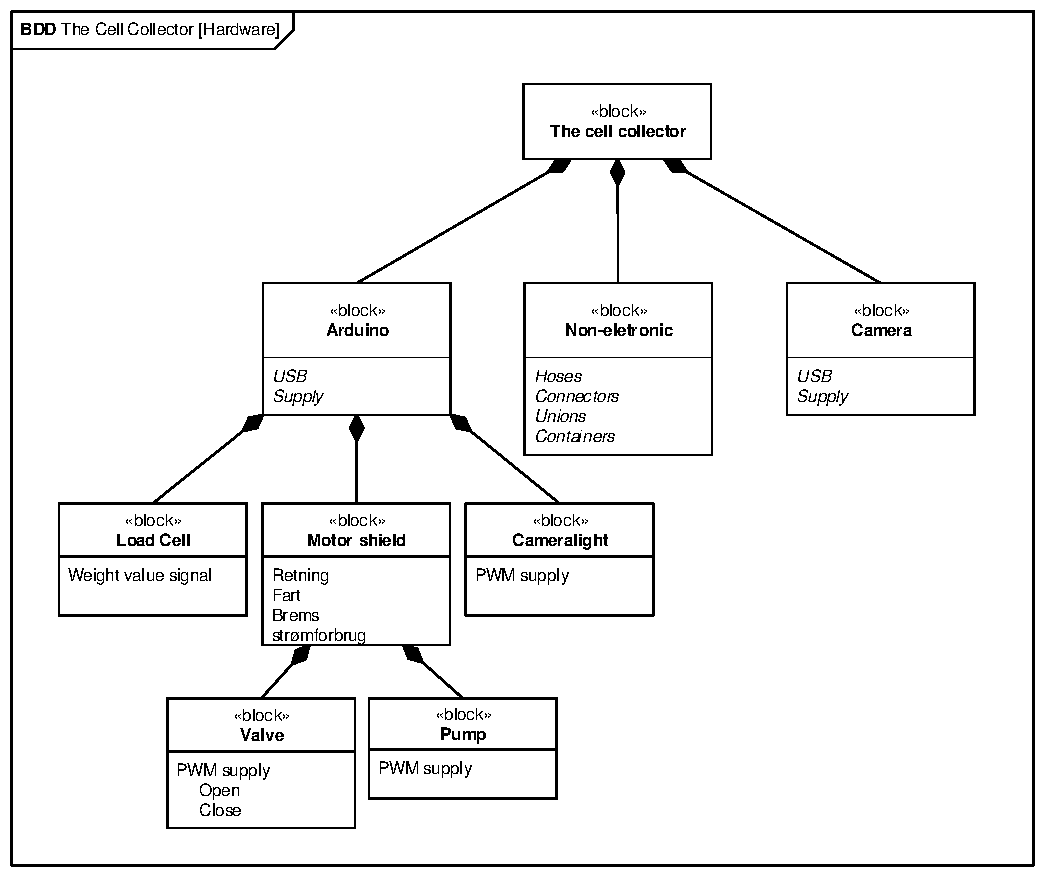
\includegraphics[width=1\textwidth]{pdf/BDD_Hardware_4315_cropped.pdf}
	\caption{BDD - Cell Collector [Hardware]}
	\label{fig:bdd_Hardware}
\end{figure}

\newpage
\subsection{Internal block Diagram} 
Et IBD diagram beskriver mere præcist, hvordan de forskellige komponenter interagerer med hinanden på. Det betyder at der er specificeret indgangs- og udgangsporte, med de forskellige typer. Digrammet(\ref{fig:ibd_Hardware}) beskriver blandt andet, hvilken spænding delene arbejder under og hvilket signal der er brug for.


\begin{figure}[H]
	\centering
	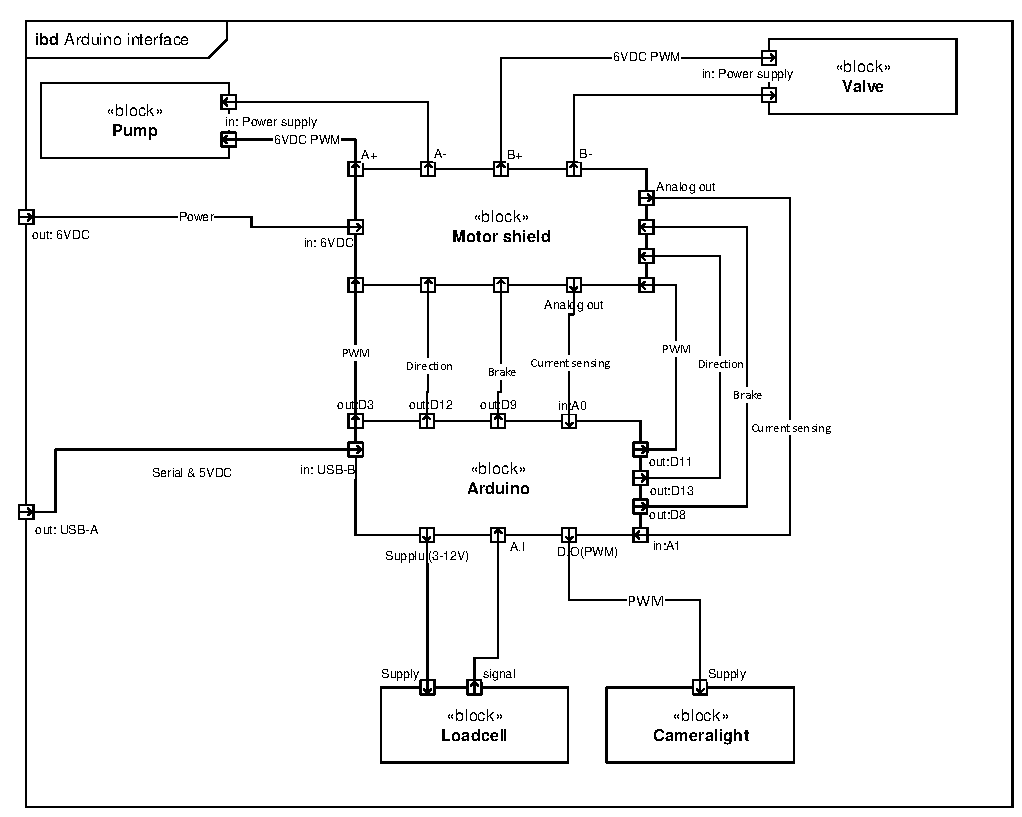
\includegraphics[width=1\textwidth]{pdf/IBD_Hardware(Arduino)_cropped.pdf}
	\caption{IBD - Cell Collector [Hardware]}
	\label{fig:ibd_Hardware}
\end{figure}

\newpage
\subsection{Kamera}
\label{subsec:Kamera}
Kameraet[\citet{DH2}] skal detektere de langerhanske øer i systemet, hvilket gør at det er en elementær del af projektet.

\textbf{Specifikationer for kameraet:} 
\begin{center}
		\begin{longtable}{ | m{6.5cm} | m{6.5cm}| } 
			\hline
			\textbf{Specifikation} &\textbf{Værdi} \\ 
			\hline
			\textbf{Billede opløsning:} & 2M Pixel \\ 
			\hline
			\textbf{Fokus område:} & 0-40mm  \\ 
			\hline
			\textbf{forstørrelse:} & 25X-400X (Manuelt)  \\ 
			\hline
			\textbf{Frame rate:} & 30f/s  \\ 
			\hline
			\textbf{Interface:} & USB 2.0  \\ 
			\hline
			\textbf{Forsyning:} & DC 5V (\textit{fra USB port})  \\ 
			\hline
			\textbf{Dimension:} & L:\SI{112}{\milli\metre} x B:\SI{33}{\milli\metre}  \\ 
			\hline			
		\end{longtable}
		
	\end{center}
Da Langerhanske øer har en størrelse på \SI{100}{\micro\metre} til \SI{300}{\micro\metre}, skal kameraet have en opløsning så øerne kan detekteres. Opløsningen på kameraet er valg ud fra:
\begin{align}
Opløsning = \frac{afstand}{objektstørrelse} = \frac{\SI{10}{\centi\metre}}{\SI{100}{\micro\metre}} 
\end{align} \citep[s.5]{DH1}
afstanden fra objektet er vurderet ud fra, hvor langt kameraet er i den absolut maksimale afstand fra øerne. Dertil skal der kunne ses flere detaljer end ned til \SI{100}{\micro\metre}, for at kunne detektere de langerhanske øer. Derfor er der valgt et kamera med en opløsning på 2M pixels. Da de Langerhanske øer er lysere og har et andet fluorescens niveau end resten af vævet vil et kamera uden farver også være anvendeligt. Da systemet skal kunne sortere 30 langerhanske øer i minuttet, er det vurderet at en standard frame rate vil være passende. Ydermere har prisen på kameraet også været vigtigt for budgettet.

%Kameraet skal detektere de langerhanske øer, når de kommer forbi i slangen.  Da de langerhanske øer skiller sig ud ved at være mere lyse end resten af vævet, vil det være underordnet om kameraet er et farve kamera. Da systemet ikke skal operere under en stor hastighed er en standard frame rate valgt på 30 f/s. Kameraet opløsningen er valgt ud fra, at det skal kunne se de langerhanske øer med en størrelse på 100-300um. Til bestemmelse til dette er der brugt følgende formel:
 %\fixme{Mangler formel}
%For at kameraet har mulighed for, at se lidt flere detaljer og forhåbning om at det kan være tættere på end 10 cm, er det besluttet er et 2 megapixels kamera burde være passende.


 
\newpage
\subsection{Microcontroller}
Microcontrolleren skal være styrerenheden i systemet, det betyder at den skal styre ventil, kameralyset, pumpe og vægtcelle.  

\textbf{Specifikationer for Microcontroller[\citet{DH3}]:} 
\begin{center}
		\begin{longtable}{ | m{6.5cm} | m{6.5cm}| } 
			\hline
			\textbf{Specifikation} &\textbf{Værdi} \\ 
			\hline
			\textbf{Type:} & Arduino UNO (ATmega328P) \\ 
			\hline
			\textbf{Forsyning:} & 5VDC (USB)  \\ 
			\hline
			\textbf{Clock speed:} & 16 MHz  \\ 
			\hline		
			\textbf{Digitale I/O pins:} & 14 stk (6 stk med PWM)  \\ 
			\hline	
			\textbf{Analoge inputs pins:} & 6 stk  \\ 
			\hline	
			\textbf{Interface:} & USB  \\ 
			\hline	
			\textbf{I/O output strøm:} & 20 mA  \\ 
			\hline
			\textbf{Flash hukommelse:} & 32 KB  \\ 
			\hline	
		\end{longtable}
\end{center}
Arduino er en open source platform til fremstilling af prototype print, med en ATmega328P microcontroller. Arduino platformen er valgt da Matlab understøtter interaktion via en Support package. Boardet er brugt i et stort omfang omkring i verden. Derfor er det en platform der er nemt tilgængelig og forholdsvis prisvenlig, samt at der findes en stor mængde dokumentation omkring emnet. Da det er en open source platform, kan der købes forskellige versioner som ikke er originaler. Arduino UNO er passende til dette system, da det er en forholdsvis simpel opgave microcontrolleren skal håndtere. Da systemet bruger computerens hukommelse og det meste er koden her på. Antallet af digitale og analoge porte er passende med den nuværende mængde af komponenter der skal styres. 

\subsection{Motor shield}
Motor shieldet skal hjælpe microcontrolleren med, at styre pumpen og ventilen til systemet. Det skal den fordi Arduinoen ikke kan trække pumpen alene, derfor skal der en ekstern forsyningskilde på, som forsynes i gennem motor shieldet. Motor shieldet skal også forsyne ventilen. 

 \textbf{Specifikationer for Motor shield[\citet{DH4}]:} 
\begin{center}
		\begin{longtable}{ | m{6.5cm} | m{6.5cm}| } 
			\hline
			\textbf{Specifikation} &\textbf{Værdi} \\ 
			\hline
			\textbf{Type:} & Velleman L298P \\ 
			\hline
			\textbf{Forsyning:} &  \fxnote{Ikke vedtaget endnu} ???)  \\ 
			\hline
			\textbf{Output spænding} & 50V (max)  \\ 
			\hline		
			\textbf{Output strøm} & 2.5A  \\ 
			\hline	
			\textbf{Kanaler} & 2 stk  \\ 
			\hline	
			\textbf{Interface} & Forsynes i gennem arduino  \\ 
			\hline	
		\end{longtable}
\end{center}
Motor shieldet kan levere 2.5A pr. kanal hvilket er nok til at forsyne pumpe og ventil. Derudover køres der PWM til den som gives videre til pumpe og ventil. Motor shieldet har desuden også den fordel, at den er galvanisk adskilt fra Arduinoen. og derved ikke kan nedlægge Arduinoen mm. Ydermere giver den også mulighed for at overvåge strømforbrugey på dens kanaler. Det kan være med til at beskytte pumpens motor.


\subsection{Ventil}
Ventilens funktion er at sortere de langerhanske øer, fra resten af opløsningen. Det gør den ved at Arduinoen giver den besked om, at åbne og lukke for ventilen.

\textbf{Specifikationer for Ventil[\citet{DH5}]:} 
\begin{center}
		\begin{longtable}{ | m{6.5cm} | m{6.5cm}| } 
			\hline
			\textbf{Specifikation} &\textbf{Værdi} \\ 
			\hline
			\textbf{Type:} & Solenoid Electromagnet Valve \\ 
			\hline
			\textbf{Forsyning:} & 6VDC, 0.3A  \\ 
			\hline
			\textbf{Porte} & 3 stk \\ 
			\hline		
			\textbf{studser} & 4mm  \\ 
			\hline	
			\textbf{Interface} & open/closed  \\ 
			\hline	
		\end{longtable}
\end{center}
Ventilen er en vigtig del af systemets hardware, da det er dens ansvar at sortere de detekterede øer fra resten af væsken. Det er svært at finde ventiler med \SI{500}{\micro\metre} studser. Det kan godt lade sig gøre at få adaptere så større ventiler kan bruges, men sporbarheden omkring hvor den enkelte ø befinder sig, forsvinder hvis kammeret pludseligt bliver stort. Der er utrolig stor variation i kvalitet og pris på magnetventiler. Ventilen er et hardware, hvor der kan bruges meget tid og mange penge i projektet.
Kravene til ventilen er, at den skal være 3 vejs med 1 tilgang og 2 udgange, yderligere skal studserne kunne tilpasses slange størrelsen, være til væske og have en lukke/åbne tid under 50 ms.

\newpage
\subsection{Pumpe}
Pumpen skal skabe det nødvendige flow i væsken fra det ene punkt til det andet. Flowet skal være lavt nok til at kameraet kan nå at detekterer en ø.

\textbf{Specifikationer for Pumpe[\citet{DH8}]:} 
\begin{center}
		\begin{longtable}{ | m{6.5cm} | m{6.5cm}| } 
			\hline
			\textbf{Specifikation} &\textbf{Værdi} \\ 
			\hline
			\textbf{Type:} & Peristaltisk pumpe \\ 
			\hline
			\textbf{Forsyning:} & 6VDC, ?A  \\ 
			\hline
			\textbf{Hastighed} & 0.1-60 omdr./.(0-60ml./min.) \\ 
			\hline		
			\textbf{studser} & variable slange størrelse  \\ 
			\hline	
		\end{longtable}
\end{center}

Det er et krav at pumpens flow hastighed er variabel, så flowet kan justeres. Der findes mange forskellige pumpetyper til formålet, herunder stempel pumper, peristaltiske pumper og vakuum pumper. Der er bestilt en peristaltisk pumpe som virker ved at klemme på slangen og derved skabe et flow, det skal dog undersøges hvordan de langerhanske øer vil opfører sig ved sådan en pumpe.
% Der er også købt en vakuum pumpe, som muligvis kan sidde efter ventilen. Der skal dog stadig skabes et flow til de sorterede øers beholder, måske en kombination vil være det optimale. En modultest af de enkelte pumper skal afgøre hvilken løsning der er den mest optimale. 

\subsection{Vægtcelle}
Vægtcellen skal bruges til at kontrollere om, der er væske i celleopløsningsbeholderen.

\textbf{Specifikationer for Vægtcelle[\citet{DH7}]:} 
\begin{center}
		\begin{longtable}{ | m{6.5cm} | m{6.5cm}| } 
			\hline
			\textbf{Specifikation} &\textbf{Værdi} \\ 
			\hline
			\textbf{Max belastning:} & 1 kg \\ 
			\hline
			\textbf{Anbefalet arbejdsspænding} & 3-12V \\ 
			\hline
			\textbf{Output} & 1.0mV/V+10.15mV/V \\ 
			\hline
		\end{longtable}
\end{center}

Den indkøbte vægtcellen kan veje op til 1 kg, hvilket fint dækker vægten for celleopløsningsbeholderen på 250ml + beholderens vægt.


%Det vil sige hvs operatøren ikke har fyldt noget i beholderen, kan der gives en systembesked omkring dette. Det mest optimale er at der hele tiden er væske i slangerne i systemet, det er det vægtcellen skal hjælpe med.

\newpage
\subsection{Beholdere}
Systemet består af tre beholdere der hver i især har sin egen funktion. Den første kaldes \textit{celleopløsningbeholderen}, som skal indeholde den usorteret opløsning med de langerhanske øer. Beholder nummer to kaldes \textit{isolerede beholderen}, som er den beholder hvor de isolerede langerhanske øer samles i. Den tredje beholder er \textit{waste beholderen}, den skal have resten af opløsningen som ikke består af langerhanske øer.
\begin{center}
		\begin{longtable}{ | m{6.5cm} | m{6.5cm}| } 
			\hline
			\textbf{Specifikation} &\textbf{Værdi} \\ 
			\hline
			\textbf{Type:} & Opløsningsbeholder(Mikrolab 33184) \\ 
			\hline
			\textbf{Størrelse:} & 250 ml \\ 
			\hline
		\end{longtable}
\end{center}
Størrelses kravene til beholderne er at opløsningsbeholderen skal mindst være 250ml, da det er den største mængde opløsning der vil blive brugt. Wastebeholderen skal således være dobbelt så stor, så der kan gennemløbes to sorterings cyklusser uden at skulle tømme beholderen i mellem. Den isolerede beholder, skal kunne rumme mængden af de isolerede øer. Da projektet som tidligere nævnt er et ”proof of concept” er den eneste beholder der er hentet informationer om opløsningsbeholderen. Den bør være støvtæt, uden at være lufttæt da der ellers vil dannes et vakuum i beholderen. Derudover vil det være en fordel hvis den er forholdsvis robust, så den kan køles ned osv. på et senere tidspunkt. ML 33184 fås med et skruelåg med forskruninger, der kan tilpasses de indkøbte slanger. Yderligere fås den et luftfilter, så der ikke dannes vakuum i beholderen.

\subsection{Slanger}
Slangerne anvendes til at føre opløsningen med de langerhanske øer, i gennem systemet bl.a. forbi kameraet.

\textbf{Specifikationer for Slangerne:(flere)} 
\begin{center}
		\begin{longtable}{ | m{6.5cm} | m{6.5cm}| } 
			\hline
			\textbf{Specifikation} &\textbf{Værdi} \\ 
			\hline
			\textbf{Materiale:} & Teflon, silikone og PVC \\ 
			\hline
			\textbf{Ydre diameter:} & ?mm  \\ 
			\hline
			\textbf{Indre diameter:} & \SI{500}{\micro\metre}-\SI{700}{\micro\metre}  \\ 
			\hline			
		\end{longtable}
\end{center}

Da de største langerhanske øer, som systemet skal håndtere er \SI{300}{\micro\metre} i diameter, derfor er det valgt at slangerne skal have en indre diameter på \SI{500}{\micro\metre}. Da det er optimalt at kameraet kan se direkte igennem slangen, er der valgt et gennemsigtigt materiale. Yderdiameteren er valgt for at, pumpen ikke skal ødelægge celler og slange, hvilket også har været med til at bestemme materialet af slangerne. 

\subsection{Glasrør}
For at sikre, at kameraet er i stand til at se de langerhanske øer, er der valgt et glasrør.

\textbf{Specifikationer for Glasrøret:} 
\begin{center}
		\begin{longtable}{ | m{6.5cm} | m{6.5cm}| } 
			\hline
			\textbf{Specifikation} &\textbf{Værdi} \\ 
			\hline
			\textbf{Materiale:} & glas \\ 
			\hline
			\textbf{Ydre diameter:} & ?mm  \\ 
			\hline
			\textbf{Indre diameter:} & \SI{500}{\micro\metre}-\SI{700}{\micro\metre}  \\ 
			\hline			
		\end{longtable}
\end{center}
Glasrøret er tiltænkt kun til at sidde, hvor kameraet skal detektere de langerhanske øer. For at være sikker på at kameraet kan se dem. Glasrøret der er valgt er rundt. Krumningen i røret kan muligvis ændre billedet fra kameraet. Et rektangel glasrør har været overvejet, men risikoen for at de langerhanske øer kan overhale hinanden inden i er for stor. Derfor er et rundt glasrør valgt.





